\documentclass[a4paper]{article}

%Tutti gli usepackage vanno qui

\usepackage{geometry}
\usepackage[italian]{babel}
\usepackage[utf8]{inputenc}
\usepackage[T1]{fontenc}
\usepackage{tgschola}
%\usepackage{tgbonum}
\usepackage{tabularx}
\usepackage{longtable}
\usepackage{hyperref}
\usepackage{enumitem}
\usepackage[toc]{appendix}
\hypersetup{
	colorlinks=true,
	linkcolor=black,
	filecolor=magenta,      
	urlcolor=blue,
}
% Numerazione figure 
\let\counterwithout\relax
\let\counterwithin\relax
\usepackage{chngcntr}

\counterwithin{table}{subsection}
\counterwithin{figure}{subsection}

\usepackage[bottom]{footmisc}
\usepackage{fancyhdr}
\setcounter{secnumdepth}{4}
\usepackage{amsmath, amssymb}
\usepackage{array}
\usepackage{graphicx}

\usepackage{ifthen}

%\usepackage{float}
\usepackage{layouts}
\usepackage{url}
\usepackage{comment}
\usepackage{float}
\usepackage{eurosym}

\usepackage{lastpage}
\usepackage{layouts}
\usepackage{float}
\usepackage{eurosym}

%Comandi di impaginazione uguale per tutti i documenti
\pagestyle{fancy}
\lhead{
\includegraphics[scale=0.04]{../../../../latex/images/logoTWM.png}}
%Titolo del documento
\rhead{\doctitle{}}
%\rfoot{\thepage}
\cfoot{Pagina \thepage\ di \pageref{LastPage}}
\setlength{\headheight}{35pt}
\setcounter{tocdepth}{5}
\setcounter{secnumdepth}{5}
\renewcommand{\footrulewidth}{0.4pt}

% multirow per tabelle
\usepackage{multirow}

% Permette tabelle su più pagine
%\usepackage{longtable}


% colore di sfondo per le celle
\usepackage[table]{xcolor}

%COMANDI TABELLE
\newcommand{\rowcolorhead}{\rowcolor[HTML]{9b240a}} %intestazione 
% check for missing commands
\newcommand{\headertitle}[1]{\textbf{\color{white}#1}} %titolo colonna
\definecolor{pari}{HTML}{FFDBCB}
\definecolor{dispari}{HTML}{F1F7FD}

% comandi glossario
\newcommand{\glo}{$_{G}$}
\newcommand{\glosp}{$_{G}$ }


%label custom
\makeatletter
\newcommand{\uclabel}[2]{%
	\protected@write \@auxout {}{\string \newlabel {#1}{{#2}{\thepage}{#2}{#1}{}} }%
	\hypertarget{#1}{#2}
}
\makeatother

%riportare pezzi di codice
\definecolor{codegray}{gray}{0.9}
\newcommand{\code}[1]{\colorbox{codegray}{\texttt{#1}}}



% Configurazione della pagina iniziale
\newcommand{\doctitle}{Norme di Progetto}
\newcommand{\docdate}{ } % lasciare vuoto (uno carattere di spazio) per i documenti che non sono verbali, così non viene scritta la data
\newcommand{\rev}{3.0.1}
\newcommand{\stato}{Non Approvato}
\newcommand{\uso}{Interno}
\newcommand{\approv}{--De Renzis Simone}
\newcommand{\red}{Greggio Nicolò\\& Tessari Andrea}
\newcommand{\ver}{Zuccolo Giada\\& Crivellari Alberto}
\newcommand{\dest}{Three Way Milkshake\\ Prof. Vardanega Tullio\\ Prof.
 Cardin Riccardo}
\newcommand{\describedoc}{Questo documento contiene tutte le norme di progetto\textsubscript{G}, definite inizialmente o aggiunte in seguito, viene quindi aggiornato per incrementi successivi.}



 % modifica questo file
\makeindex

\usepackage{hyperref}
\hypersetup{
    colorlinks=true,
    linkcolor=blue,
    urlcolor=blue,
    hyperfootnotes=false
}
\usepackage{multicol}
\usepackage{pgfplots}
\usepackage{verbatim}
\usepackage{pgf-pie}
\usepackage{ragged2e}
\usepackage[section]{placeins} %in teoria evita che elementi tipo tabelle rompano il flow e vadano in sezioni dopo rispetto a dove dichiarate (al momento semrba funzionare)
\usepackage{caption}


\setlength{\columnseprule}{1pt}
\newcommand{\group}{Three Way Milkshake}
\newcommand{\pparagraph}[1]{\paragraph{#1}\mbox{}\\}

\makeatletter
\renewcommand\subparagraph{%
    \@startsection {subparagraph}{5}{\z@ }{3.25ex \@plus 1ex
        \@minus .2ex}{-1em}{\normalfont \normalsize \bfseries }}%
\makeatother

\begin{document}
	\thispagestyle{empty}
\begin{titlepage}
	\begin{center}
		
		
\includegraphics[scale = 0.17]{../../../../latex/images/logoTWM.png}\\[0.7cm]
		

		\noindent\rule{\textwidth}{1pt} \\[0.4cm]
		\Huge \textbf{\doctitle} \\[0.1cm]
		\ifthenelse{\equal{\docdate}{ }}{ }{ \huge \textbf{\docdate} \\[0.1cm] }
		
		\noindent\rule{\textwidth}{1pt}\\[0.7cm]
		
		\large \textbf{Three Way Milkshake - Progetto "PORTACS"} \\[0.4cm] 
                \texttt{threewaymilkshake@gmail.com} \\[0.4cm]
                
		
        
        
        \large

        \begin{tabular}{r|l}
                        \textbf{Versione} & \rev{} \\
                        \textbf{Stato} & \stato{} \\
                        \textbf{Uso} & \uso{} \\                         
                        \textbf{Approvazione} & \approv{} \\                      
                        \textbf{Redazione} & \red{} \\ 
                        \textbf{Verifica} &  \ver{} \\                         
                        \textbf{Destinatari} & \parbox[t]{5cm}{ \dest{} }
                \end{tabular} 
                \\[0.3cm]
                \large \textbf{Descrizione} \\ \describedoc{} 
               

	\end{center}
\end{titlepage}
	\pagebreak

	% Registro delle modifiche
	\section*{Registro delle modifiche}

\newcommand{\changelogTable}[1]{
	
	
	\renewcommand{\arraystretch}{1.5}
	\rowcolors{2}{pari}{dispari}
	\begin{longtable}{ 
			>{\centering}p{0.07\textwidth} 
			>{}p{0.21\textwidth}
			>{\centering}p{0.17\textwidth}
			>{\centering}p{0.13\textwidth} 
			>{\centering}p{0.17\textwidth} 
			>{\centering}p{0.13\textwidth} }
		\rowcolorhead
		\headertitle{Vers.} &
		\centering \headertitle{Descrizione} &	
		\headertitle{Redazione} &
		\headertitle{Data red.} & 
		\headertitle{Verifica} &
		\headertitle{Data ver.}
		\endfirsthead	
		\endhead
		
		#1
		
	\end{longtable}
	\vspace{-2em}
	
}


\newcommand{\approvingTable}[1]{ 
	
	
	\renewcommand{\arraystretch}{1.5}
	\rowcolors{2}{pari}{dispari}
	\begin{longtable}{ 
			>{\centering}p{0.07\textwidth} 
			>{\centering}p{0.415\textwidth}
			>{\centering}p{0.13\textwidth}
			>{\centering}p{0.322\textwidth}  }
		\rowcolorhead
		\headertitle{Vers.} &
		\centering \headertitle{Descrizione} &	
		\headertitle{Data appr.} &
		\headertitle{Approvazione}
		\endfirsthead	
		\endhead
		
		#1
		
	\end{longtable}
	\vspace{-2em}
	
}
	\changelogTable{
	3.5.0 & Incremento appendice \S\ A e B & Crivellari Alberto & 2021-04-26 & -- & --
	3.4.0 & Rimossa appendice \S\ D & Crivellari Alberto & 2021-04-01 & -- & --
	\tabularnewline
	3.3.0 & Modifica sezioni \S\ 2 e \S\ 3 & Crivellari Alberto & 2021-04-01 & -- & --
	\tabularnewline
	3.2.0 & Modifica appendice \S\ B & Zuccolo Giada & 2021-03-31 & -- & --
\tabularnewline
	3.1.0 & Aggiornamento appendice \S\ C & Crivellari Alberto & 2021-03-20 & -- & --
}

\approvingTable{
    3.0.0 & Approvazione del documento & 2021-03-08 & Zuccolo Giada
}

\changelogTable{
    2.1.0 & Aggiornamento sezioni \S\ 4 e 5 & Crivellari Alberto & 2021-03-08 & Chiarello Sofia & 2021-03-08
}

\approvingTable{
    2.0.0 & Approvazione del documento & 2021-02-22 & De Renzis Simone
}

\changelogTable{
1.3.0 & Completamento stesura appendice \S\ D e \S\ B & Crivellari Alberto & 2021-02-12 & Greggio Nicolò & 2021-02-19
\tabularnewline
1.2.1 & Completamento stesura sezione \S\ 2 e \S\ 3 & Chiarello Sofia & 2021-02-11 & Tessari Andrea & 2021-02-13
\tabularnewline
1.2.0 & Stesura sezione \S\ 3 e appendice \S\ C & Chiarello Sofia & 2021-02-09 & Tessari Andrea & 2021-02-12
\tabularnewline
1.1.0 & Stesura sezione \S\ 2 & Chiarello Sofia & 2021-02-08 & Tessari Andrea & 2021-02-13
}

\approvingTable{
	1.0.0 & Approvazione del documento & 2021-01-10 & De Renzis Simone
}

\changelogTable{
0.5.1 & Aggiunta tabelle a sezione \S 4 e \S5 & Crivellari Alberto & 2021-01-08 & Greggio Nicolò & 2021-01-10
\tabularnewline
0.5.0 & Redazione sezione \S 5 & Crivellari Alberto & 2020-12-07 & Greggio Nicolò & 2021-01-10
\tabularnewline
0.4.0 & Redazione sezione \S 4 & Crivellari Alberto & 2020-12-06 & Greggio Nicolò & 2021-01-10
\tabularnewline
0.3.2 & Modifiche sezione \S 1 & Crivellari Alberto & 2020-12-30 & Greggio Nicolò & 2021-01-10
\tabularnewline
0.3.1 & Tabelle sezione \S 3 & Crivellari Alberto & 2020-12-29 & Greggio Nicolò & 2021-01-10
\tabularnewline
0.3.0 & Redazione sezione \S 3 & Tessari Andrea & 2020-12-28 & Greggio Nicolò & 2021-01-10
\tabularnewline
0.2.1 & Tabelle sezione \S 2 & Crivellari Alberto & 2020-12-20 &  Greggio Nicolò & 2021-01-09
\tabularnewline
0.2.0 & Redazione sezione \S 2 & Crivellari Alberto & 2020-12-19 & Greggio Nicolò & 2021-01-09
\tabularnewline
0.1.1 & Modifiche sezione \S 1  & Crivellari Alberto & 2020-12-18 & Greggio Nicolò & 2021-01-09
\tabularnewline
0.1.0 & Redazione sezione \S 1 & Crivellari Alberto & 2020-12-16 & Greggio Nicolò & 2021-01-09
\tabularnewline
0.0.1 & Strutturazione del documento & Tessari Andrea & 2020-12-15 & Greggio Nicolò & 2021-01-09
}


 % modifica questo file
	%\end{longtable}
	\pagebreak

	% indice
	{
        \hypersetup{linkcolor=black}
        \tableofcontents
        \pagebreak

        % indice delle figure
        \listoffigures
        \pagebreak

        % indice delle tabelle
        \listoftables
        \pagebreak
    }

	\newcommand{\contabilitaTable}[1]{

\begin{table}[H]
	\begin{center}
		\begin{tabular}{c
				!{\color[HTML]{9b240a}\vrule width 1pt}
				cccccc
				!{\color[HTML]{9b240a}\vrule width 1pt}	
				c}
			\rowcolorhead
			\headertitle{Nome} & \headertitle{R} & \headertitle{V} & \headertitle{An} & \headertitle{Am} & \headertitle{Pr} & \headertitle{Pt} & \headertitle{Tot} \\	
			#1
			\end{center}
			\end{table}	
}


\newcommand{\smallPreventivoTable}[1]{
	
	\begin{table}[H]
		\begin{center}
			\begin{tabular}{c
					!{\color[HTML]{9b240a}\vrule width 1pt}
					cccccc
					!{\color[HTML]{9b240a}\vrule width 1pt}	
					c}
				\rowcolorhead
				\headertitle{Ruolo} & \headertitle{Tempo (ore)} & \headertitle{Costo (\euro)} \\
				#1
			\end{center}
		\end{table}	
	}


\newcommand{\planningTable}[1]{
	
	
	\renewcommand{\arraystretch}{1.5}
	\rowcolors{2}{pari}{dispari}
	\begin{longtable}{ 
			>{}p{0.25\textwidth} 
			>{}p{0.42\textwidth}
			>{\centering}p{0.05\textwidth}
			>{\centering}p{0.17\textwidth} }
		\rowcolorhead
		\headertitle{Attività} &
		\headertitle{Descrizione} &	
		\headertitle{Ore} &
		\headertitle{Ruolo} 
		\endfirsthead	
		\endhead
		#1		
	\end{longtable}
	
}


\newcommand{\pafTable}[1]{
	
	
	\renewcommand{\arraystretch}{1.5}
	\rowcolors{2}{pari}{dispari}
	\begin{longtable}{ 
			>{}p{0.40\textwidth} 
			>{\centering}p{0.10\textwidth}
			>{\centering}p{0.20\textwidth}
			>{\centering}p{0.15\textwidth} }
		\rowcolorhead
		\headertitle{Fase} &
		\headertitle{Periodo} &	
		\headertitle{Descrizione} &
		\headertitle{Spesa (\euro)} 
		\endfirsthead	
		\endhead
		#1		
	\end{longtable}
	
}


 % file con template tabelle con macro


	% contenuto del documento, ogni sezione in un file
	\section{Introduzione}
\subsection{Scopo del documento}
    Questo documento ha lo scopo di fissare e definire tutte le regole, convenzioni e buone pratiche utili a formare un way of working condiviso alla base da tutti i componenti del gruppo per assicurare una collaborazione efficiente ed efficace. Si discuteranno inoltre i vari strumenti che verranno adottati per facilitare lo sviluppo del progetto\textsubscript{G} e per promuovere un'organizzazione adeguata.
    Si ritiene inoltre che la definizione ed il mantenimento per incremento di un documento condiviso all'interno del gruppo di lavoro, che definisca e raccolga quanto descritto in maniera formale e centralizzata, possa favorire, in un contesto dove i membri possano variare, l'inserimento di nuovi componenti facilitandone l'ambientamento. Pur non essendo questo il contesto di lavoro attuale, è comunque una buona pratica da sperimentare e consolidare.

\subsection{Scopo del prodotto}
Il capitolato\textsubscript{G} C5 propone un progetto\textsubscript{G} in cui viene richiesto lo sviluppo di un software per il monitoraggio in tempo reale di unità che si muovono in uno spazio definito. All'interno di questo spazio, creato dall'utente per riprodurre le caratteristiche di un ambiente reale, le unità dovranno essere in grado di circolare in autonomia, o sotto il controllo dell'utente, per raggiungere dei punti di interesse posti nella mappa.  La circolazione è sottoposta a vincoli di viabilità e ad ostacoli propri della topologia dell'ambiente, deve evitare le collisioni con le altre unità e prevedere la gestione di situazioni critiche nel traffico.

\subsection{Termini, abbreviazioni ed altri documenti}
    Tutti i termini che necessitano di una spiegazione, per fornire un'adeguata comprensione, o perché possono causare ambiguità nel contesto, sono definiti nel glossario. A dispetto di tutti gli altri documenti presenti, il glossario è sotto la veste di una pagina web, più nello specifico in una wiki\textsubscript{G} di GitHub, accessibile a \href{https://github.com/Three-Way-Milkshake/docs/wiki/Glossario}{questo indirizzo}, con vocaboli suddivisi tra "Acronimi" e "Termini", disposti in ordine alfabetico al fine di facilitare la navigazione. All'interno dei documenti le voci di glossario saranno seguite da una G pedice mentre gli acronimi da una A (e.g.: voce di glossario\textsubscript{G} ; acronimo\textsubscript{A}).
    Inoltre quando si farà riferimento ad un altro documento o al documento stesso, il nome di questo sarà in maiuscoletto (e.g.: \textsc{esempio nome documento}).

\subsection{Riferimenti}
\label{ref}
    \subsubsection{Riferimenti Normativi}
        \begin{itemize}
            \item Standard ISO 12207:\\ \url{https://www.math.unipd.it/~tullio/IS-1/2009/Approfondimenti/ISO_12207-1995.pdf};
            \item Standard UML\textsubscript{A} 2.0:\\\url{https://www.omg.org/spec/UML/2.0/Superstructure/PDF};
            \item Diagrammi dei casi d'uso\textsubscript{G}:\\\url{https://www.math.unipd.it/~rcardin/swea/2021/Diagrammi\%20Use\%20Case_4x4.pdf};
            \item Diagrammi delle classi:\\\url{https://www.math.unipd.it/~rcardin/swea/2021/Diagrammi\%20delle\%20Classi_4x4.pdf};
            \item Diagrammi dei package:\\\url{https://www.math.unipd.it/~rcardin/swea/2021/Diagrammi\%20dei\%20Package_4x4.pdf};
            \item Diagrammi di attività\textsubscript{G}:\\\url{https://www.math.unipd.it/~rcardin/swea/2021/Diagrammi\%20di\%20Attivit\%c3\%a0_4x4.pdf};
            \item Diagrammi di sequenza:\\\url{https://www.math.unipd.it/~rcardin/swea/2021/Diagrammi\%20di\%20Sequenza_4x4.pdf};
            \item Standard ISO 8601:\\\url{https://www.iso.org/iso-8601-date-and-time-format.html}.
        \end{itemize}

    \subsubsection{Riferimenti Informativi}
        \begin{itemize}
        	\item \textsc{\href{https://github.com/Three-Way-Milkshake/docs/wiki/Glossario}{Glossario}}:\\per la definizione dei termini (pedice G) e degli acronimi (pedice A) evidenziati nel documento;
            \item \url{https://www.math.unipd.it/~tullio/IS-1/2020/Dispense/L03.pdf}
            \item \url{https://www.math.unipd.it/~tullio/IS-1/2020/Dispense/L06.pdf}
            \item \url{https://www.math.unipd.it/~tullio/IS-1/2020/Dispense/FC2.pdf}
            \item \url{https://www.math.unipd.it/~rcardin/swea/2021/SOLID\%20Principles\%20of\%20Object-Oriented\%20Design_4x4.pdf}
            \item \url{https://www.math.unipd.it/~tullio/IS-1/2020/Dispense/L09.pdf}
            \item \url{https://docs.github.com/en/free-pro-team@latest/actions}
            \item \url{https://www.latex-project.org/}
            \item \url{http://www.texstudio.org/}
            \item \url{https://www.xm1math.net/texmaker/}
            \item \url{https://www.atlassian.com/git/tutorials/comparing-workflows/gitflow-workflow}
            \item \url{https://github.com/about}
            \item \url{https://www.atlassian.com/software/jira}
            \item \url{https://www.atlassian.com/}
            \item \url{https://meet.google.com/}
            \item \url{https://slack.com/intl/en-it/about}
            \item \url{https://telegram.org/}
            \item \url{https://workspace.google.com/products/chat/}
        \end{itemize}

\pagebreak
 %@Tex
	\pagebreak

	\section{Tecnologie e librerie}

Nelle sezioni che seguono, vengono elencate le tecnologie e le librerie interessate dallo sviluppo del software. Per ognuna, viene presentata una breve descrizione e spiegato il suo impiego nel contesto del software. Dove necessario, viene fornito un collegamento per il download e l'installazione delle risorse necessarie per lo sviluppo e manutenzione del progetto.




















 %@Simone - intro

	\subsection{Server}

\subsubsection{Tecnologie}

\begin{itemize}
	\item \textbf{Java}
	\item \textbf{Json}
	\item \textbf{Docker}
	\item \textbf{Gradle}
\end{itemize}

\subsubsection{Librerie e Framework}

\begin{itemize}
	\item \textbf{Spring}
	\item \textbf{Gson}
	\item \textbf{Junit}
	\item \textbf{Mockito}

\end{itemize} %@Simone

	\subsection{Client}

\subsubsection{Tecnologie}

\begin{itemize}
	\item \textbf{Node.js}: runtime system open source multipiattaforma orientato agli eventi per l'esecuzione di codice Javascript. Molti dei suoi moduli base sono scritti in Javascript. 
	\begin{itemize}
		\item Versione utilizzata: 14.15.5
		\item Link per download: \url{https://nodejs.org/it/download/}
	\end{itemize}
	
	\item \textbf{HTML}: linguaggio markup per la strutturazione di pagine web. Viene utilizzato insieme ad Angular per la costruzione della struttura della web app.

	\item \textbf{CSS}: linguaggio utilizzato per definire la formattazione di documenti HTML, XHTML e XML, ad esempio i siti web e le relative pagine web. L'uso del CSS permette la separazione dei contenuti delle pagine HTML dal loro layout e permette una programmazione più chiara e facile da utilizzare, sia per gli autori delle pagine stesse sia per gli utenti, garantendo contemporaneamente anche il riutilizzo di codice ed una sua più facile manutenzione. Viene utilizzato insieme ad Angular per la stilizzazione degli elementi HTML.
	\item \textbf{Typescript}: linguaggio di programmazione open-source. Si tratta di un super-set di JavaScript che basa le sue caratteristiche su ECMAScript 6. Il linguaggio estende la sintassi di JavaScript in modo che qualunque programma scritto in JavaScript sia anche in grado di funzionare con TypeScript senza nessuna modifica. È progettato per lo sviluppo di grandi applicazioni ed è destinato a essere compilato in JavaScript per poter essere interpretato da qualunque web browser o app. Viene utilizzato insieme ad Angular per la codifica del comportamento della webapp.
	\begin{itemize}
		\item Versione utilizzata: 3.8 o superiore.
	\end{itemize}

\end{itemize}

\subsubsection{Librerie e Framework}

\begin{itemize}
	\item \textbf{Angular}: framework\textsubscript{G} open source per lo sviluppo di applicazioni web a single page. Esso si basa sul pattern MVVM. Si basa sul linguaggio di programmazione TypeScript e sulla creazione di componenti che costruiscono la pagina web. Le applicazioni sviluppate in Angular vengono eseguite interamente dal web browser dopo essere state scaricate dal web server (elaborazione lato client). Questo comporta il risparmio di dover spedire indietro la pagina web al web-server ogni volta che c'è una richiesta di un'azione da parte dell'utente.
	\begin{itemize}
		\item Versione utilizzata: 11.2.0
		\item Link per installazione: \url{https://angular.io/guide/setup-local}
	\end{itemize}
 	\item \textbf{PrimeNG}: libreria per Angular per personalizzare i componenti così da creare un'interfaccia utente più accattivante.
	 \begin{itemize}
		\item Link per installazione: \url{https://primefaces.org/primeng/showcase/#/setup}
	\end{itemize}

	
\end{itemize} %@TeamFE

	\subsection{Version Control System e Continuous Integration}

\subsubsection{Git e gitflow}
Git è un sistema di controllo per il versionamento veloce ed efficiente\textsubscript{G}. Gitflow è un workflow che aiuta lo sviluppo software dando delle linee guida sui branch che strutturano le repo\textsubscript{A} e le operazioni per l'implementazione di feature e rilascio di releases.\\
Maggiori informazioni:
\begin{itemize}
    \item \textbf{Git: }\url{https://git-scm.com/};
    \item \textbf{gitflow: }\url{https://www.atlassian.com/git/tutorials/comparing-workflows/gitflow-workflow}.
\end{itemize}

\subsubsection{GitHub}
GitHub è un provider di hosting internet per lo sviluppo di software e il controllo della versione utilizzando Git. Fornisce un intero ecosistema di strumenti (version control, issue tracking, project boards, continuous integration\textsubscript{G} e delivery...) e permette la creazione di account personali o di organizzazioni.
\begin{itemize}
    \item \textbf{Maggiori informazioni su GitHub:} \url{https://github.com/about};
    \item \textbf{\group{} su GitHub: }\url{https://github.com/Three-Way-Milkshake}.
\end{itemize}

\subsubsection{GitHub Actions}
È uno strumento integrato in ogni repo\textsubscript{A} di GitHub, permette di creare singole attività\textsubscript{G} combinabili al fine di realizzare complessi workflow personalizzati. 
Si possono creare nuove \textit{actions} ed eventualmente pubblicarle, o utilizzare il vasto catalogo di automazioni già realizzate dalla community.
\begin{itemize}
    \item \textbf{Documentazione: } \url{https://docs.github.com/en/actions}.
\end{itemize} %@Gregg - fatto

	\pagebreak


	\section{Setup}
PORTACS viene distribuito tramite container Docker, per cui i dispositivi sui quali dovrà eseguire avranno minimi requisiti software. È possibile utilizzare i container anche per la fase\textsubscript{G} di sviluppo, altrimenti si possono scaricare ed utilizzare gli strumenti descritti in \ref{tecnologie} per l'esecuzione diretta in locale. PORTACS\textsubscript{A} si divide su tre immagini Docker:
\begin{enumerate}
    \item server;
    \item client muletto (forklift);
    \item client utente (user).
\end{enumerate}


\subsection{Requisiti di sistema}
Sotto elencati saranno descritti i requisiti minimi del sistema per un corretto funzionamento del software PORTACS\textsubscript{A}.


\subsubsection{Requisiti Hardware}
\begin{itemize}
	\item Client → unità:
\begin{itemize}
	\item CPU\textsubscript{A} dual-core o maggiore con frequenza indicativa >= 3 Ghz;
	\item memoria RAM\textsubscript{A} >= 4GB dedicati;
	\item connessione con bassi tempi di risposta.
\end{itemize}
	\item Client → admin o responsabile:
\begin{itemize}
	\item CPU\textsubscript{A} dual-core o maggiore con frequenza indicativa >= 3 Ghz;
	\item memoria RAM\textsubscript{A} >= 4GB dedicati;
	\item connessione con bassi tempi di risposta.
\end{itemize}
	\item Server:
\begin{itemize}
	\item CPU\textsubscript{A} quad-core o maggiore con frequenza indicativa >= 4 Ghz;
	\item memoria RAM\textsubscript{A} >= 8GB dedicati;
	\item connessione con bassi tempi di risposta.
\end{itemize}
\end{itemize}

\subsubsection{Requisiti Software}
	\begin{comment}
        \pparagraph{Librerie}
        \begin{itemize}
        \item express (v4.17.1);
        \item http (v0.0.1-security);
        \item mocha (v8.3.2);
        \item net (v1.0.2);
        \item primeicons (v4.1.0);
        \item primeng (v11.3.2);
        \item rxjs (v6.6.0);
        \item socket.io (v3.1.2);
        \item spring boot (v2.4.5).
        \end{itemize}
    \end{comment}

    \pparagraph{Esecuzione}
    \begin{itemize}
   		\item Utilizzando Docker, il sistema operativo host non dovrebbe essere un problema, tuttavia in seguito si daranno le istruzioni per l'esecuzione valide in ambiente unix, nel quale si è anche effettuato la maggior parte dei test (Linux kernel v5.8 o MacOS v10.15);
        \item Docker (v19.03.*), installazione base, per esempio in Linux è sufficiente: \texttt{sudo snap install docker};
        \item Google Chrome (v90).
    \end{itemize}

    \pparagraph{Sviluppo}
    Vedi \S\ \ref{tecnologie}

    \begin{comment}
    	\item Client:
    \begin{itemize}
    	\item Docker.
    	%\item Chrome Versione 90.0.4430.85 (Build ufficiale) (a 64 bit);
    	%\item Node.js;
    	%\item Angular;

    	%\item Windows 10.
    \end{itemize}
    	\item Server:
    \begin{itemize}
    	\item Docker.
    	%\item Java;
    	%\item gradle;

    	%\item Windows 10.
    \end{itemize}
    \end{comment}







\subsection{Installazione ed avvio degli applicativi}
    \subsubsection{Server}
    Nella macchina da utilizzare come server andrà scaricata l'immagine di portacs-server con la versione desiderata dal \href{https://hub.docker.com/r/threewaymilkshake}{docker hub di \group}.
    Per l'avvio, in ambiente Linux e MacOS:
    \begin{itemize}
        \item predisporre una cartella nella quale posizionarsi per l'esecuzione che contenga una cartella \texttt{database} che manterrà la persistenza, questa dovrà contenere i file \texttt{map.json}, \texttt{forklifts.json} e \texttt{users.json};
        \item posizionarsi su tale cartella;
        \item eseguire:
    \begin{verbatim}
    docker run --rm --name server \
        -v $(pwd)/database:/database \
        -p 1723:1723 \
        threewaymilkshake/portacs-server
    \end{verbatim}
    \end{itemize}
    Il container verrà avviato nella finestra corrente e si potranno osservare i log del server, questo può essere terminato dalla stessa finestra con la combinazione \texttt{Ctrl+C}. Se si vuole eseguire il container in background è sufficiente aggiungere l'opzione \texttt{-d}, per terminarlo a questo punto bisognerà eseguire: \texttt{docker stop server}.
    Si raccomanda di impostare un ip statico per la macchina server, così da non dover richiedere variazioni frequenti nelle configurazioni dei client.

    \subsubsection{Client}
    Come per il server, scaricare l'immagine dal \href{https://hub.docker.com/r/threewaymilkshake}{docker hub di \group{}} relativa al client voluto (forklift o user). Dopodiché posizionarsi in una cartella dove predisporre un file di configurazione \texttt{config.txt}:
    \begin{itemize}
        \item per i client \textit{user} sarà sufficiente specificare l'indirizzo IP della macchina server così: \texttt{SERVER\_ADDR=ip};
        \item per i client \texttt{forklift}, oltre all'indirizzo del server come per gli utenti, bisognerà aggiungere altre informazioni:
        \begin{itemize}
            \item \textbf{obbligatorie: }
            \begin{itemize}
                \item id e token del muletto;
                \item posizione iniziale (corrispondendte alla base dove il muletto verrà posizionato al primo avvio);
            \end{itemize}
            \item \textbf{opzionali: }
            \begin{itemize}
                \item per specificare delle porte diverse da far utilizzare ai servizi, quest'operazione è necessaria solo se si vogliono simulare più unità nella stessa macchina locale, al fine di evitare collisioni tra le porte;
                \item bisogna impostare due campi, \texttt{ngPort1} e \texttt{ngPort2}, devono essere diversi da altre configurazioni in uso sulla stessa macchina;
                \item bisogna predisporre un file diverso per ogni unità che si vuole simulare.
            \end{itemize}
        \end{itemize}
        Dev'essere poi sempre presente \texttt{configurationEnv=custom}. L'ordine in cui vengono specificati i campi non è importante. Segue un esempio di configurazione ben formata con utilizzo delle impostazioni opzionali:
        \begin{verbatim}
            startX=0
            startY=1
            ngPort1=4203
            ngPort2=8083
            forkliftId=f3
            forkliftToken=abc
            configurationEnv=custom
            SERVER_ADDR=192.168.3.129
        \end{verbatim}
        Queste informazioni sono a disposizione degli admin.
    \end{itemize}

    Per avviare un muletto sarà sufficiente eseguire (i valori di default per \texttt{ngPort1} e \texttt{ngPort2} sono rispettivamente \texttt{4201} e \texttt{8081}):
    \begin{verbatim}
        docker run --rm --name <nome> -d \
            --env-file config.txt
            -p 4201:4201 \
            -p 8081:8081 \
            portacs-client-forklift
    \end{verbatim}
    Il <nome> specificato dopo \texttt{---name} servirà per terminare il container.

    Per avviare un utente invece:
    \begin{verbatim}
        docker run --rm --name user -d \
            --env-file user.txt \
            -p 4300:4300 \
            -p 8090:8090 \
            portacs-client-user
    \end{verbatim}

    \pparagraph{Terminazione dei container}
        Se si vuole terminare un container l'istruzione è: \texttt{docker stop <nome>}, dove <nome> è il parametro che si ha specificato dopo \texttt{---name}. La specifica del nome all'avvio del container non è obbligatoria, nel caso di esecuzione con opzione \texttt{-d} verrà stampato l'id che si potrà usare al posto del nome per terminare il container o in ogni caso si possono ispezionare i container attivi tramite \texttt{docker ps}.

\clearpage
\subsection{Costruzione degli artefatti e delle immagini}
    Quando il codice sorgente viene modificato le immagini docker corrispondenti devono essere ricostruite e prima di ciò bisogna produrre gli artefatti necessari. Per le operazioni descritte in seguito si assume di avere le cartelle con i sorgenti relativi.
    \subsubsection{Server}
        Per produrre l'unico artefatto\textsubscript{G} jar necessario, si deve eseguire \texttt{./gradlew build}, questo produrrà appunto l'eseguibile segnandolo con la versione specificata in \texttt{build.gradle}. Questo comando esegue anche tutti i test di unità segnalando eventuali fallimenti. La build ha come precondizione\textsubscript{G} la corretta formattazione del codice, la quale può essere ottenuta con \texttt{./gradlew spotlessApply}.
        Con il jar aggiornato si può eseguire la build di docker per ottenere l'immagine aggiornata:
        \begin{verbatim}
            docker build -t threewaymilkshake/portacs-server .
        \end{verbatim}

    \subsubsection{Client}
        Per entrambi i client bisogna assicurarsi che il file \texttt{node\_package.json} nelle cartelle corrispondenti contenga tutte e sole le dipendenze necessarie a node. Dopodiché bisogna compilare la parte angular:
        \begin{itemize}
            \item per i muletti: \texttt{ng build -c dev1};
            \item per gli utenti: \texttt{ng build}.
        \end{itemize}
        A questo punto si possono generare le rispettive immagini:
        \begin{verbatim}
            docker build -t threewaymilkshake/portacs-client-forklift .
            docker build -t threewaymilkshake/portacs-client-user .
        \end{verbatim}


    \subsubsection{Caricamento nel docker hub}
        \noindent Per aggiornare le immagini nel docker hub, è necessario avere le credenziali o essere collaboratori. Dopo aver effettuato l'accesso tramite tramite \texttt{docker login}, è sufficiente eseguire: \texttt{docker {push} <nome-immagine>}












 %TODO
	\pagebreak


	\section{Testing}
Questo capitolo ha lo scopo di indicare agli sviluppatori come controllare in che modo opera il codice e la sua sintassi. Vengono di seguito esposti gli strumenti utilizzati per effettuare i test di analisi statica e dinamica del nostro applicativo.

\subsection{Coveralls}
Per quanto riguarda l'attività di code coverage è stato scelto di utilizzare \textit{Coveralls}. \textit{Coveralls} esegue revisioni automatiche al codice relative all'analisi statica attraverso \textit{GitHub Actions}.

\subsection{GitHub Actions}
Il servizio di Continuous Integration che è stato deciso di utilizzare è \textit{GitHub Actions}, fornito da \textit{GitHub}. \\\textit{GitHub Actions} permette di creare dei workflow, ovvero processi automatici, con l'obiettivo di automatizzare il ciclo di vita dello sviluppo del software.

% CI e code coverage, glossario



 %@Alberto

	\subsection{Testing lato server}
\subsubsection{Junit}
Un framework di unit testing per la programmazione java. Junit viene utilizzato per i test di unità relativi al codice in Java.
Per effettuare i test basterà eseguire il comando ./gradlew test.

\subsubsection{Spring}
Framework utilizzato per la risoluzione delle dipendenze e come supporto durante la scrittura degli unit test. %@Alberto (aiuto di teamBE)

	\subsection{Testing lato client}

\subsubsection{Jasmine}
Jasmine è un framework di unit testing per il codice JavaScript.
Viene utilizzato per i test di unità relativi al codice in Angular CLI.
Si scrivono i test, in un formato leggibile ad occhio umano, e si eseguono attraverso dei file formato js, collegati a relativi file html e css.

\subsubsection{Karma}
Karma è un test runner, che permette di utilizzare Jasmine in maniera più efficace.
Karma e Jasmin vengono utilizzati in quanto framework di default per unit testing di Angular CLI.

\subsubsection{Mocha}
Mocha è un framework di unit testing per il codice JavaScript.
Viene utilizzato per i test di unità relativi al codice in NodeJS. %@Alberto (aiuto di teamFE)

	\pagebreak


	\section{Architettura del sistema}


Qui si potrebbe mettere uno schema simile a quello della slide iniziale per evidenziare l'architettura client-server



\subsection{Server}

Dire che è 3 layer architecture

Qui potrebbe esserci il diagramma minimale complessivo


\subsubsection{Diagramma delle classi}


\paragraph{Persistance layer}


\paragraph{Business layer}

\subparagraph{Mappa}

\subparagraph{Clients}

\subparagraph{Tasks}

\subparagraph{Collisioni}


\paragraph{Communication layer}



\subsection{Client}


\subsection{Comunicazione}

\subsubsection{Diagrammi di sequenza}

\subsubsection{Protocollo di comunicazione}


 %@Simone - %Intro

	\subsection{Server}

L'architettura della componente server si articola in una 3-layer architecture, in cui si identificano i seguenti layer:
\begin{itemize}
	\item \textbf{Communication layer}
	\item \textbf{Business layer}
	\item \textbf{Persistence layer}
\end{itemize}

\begin{figure}[H]
	\centering
	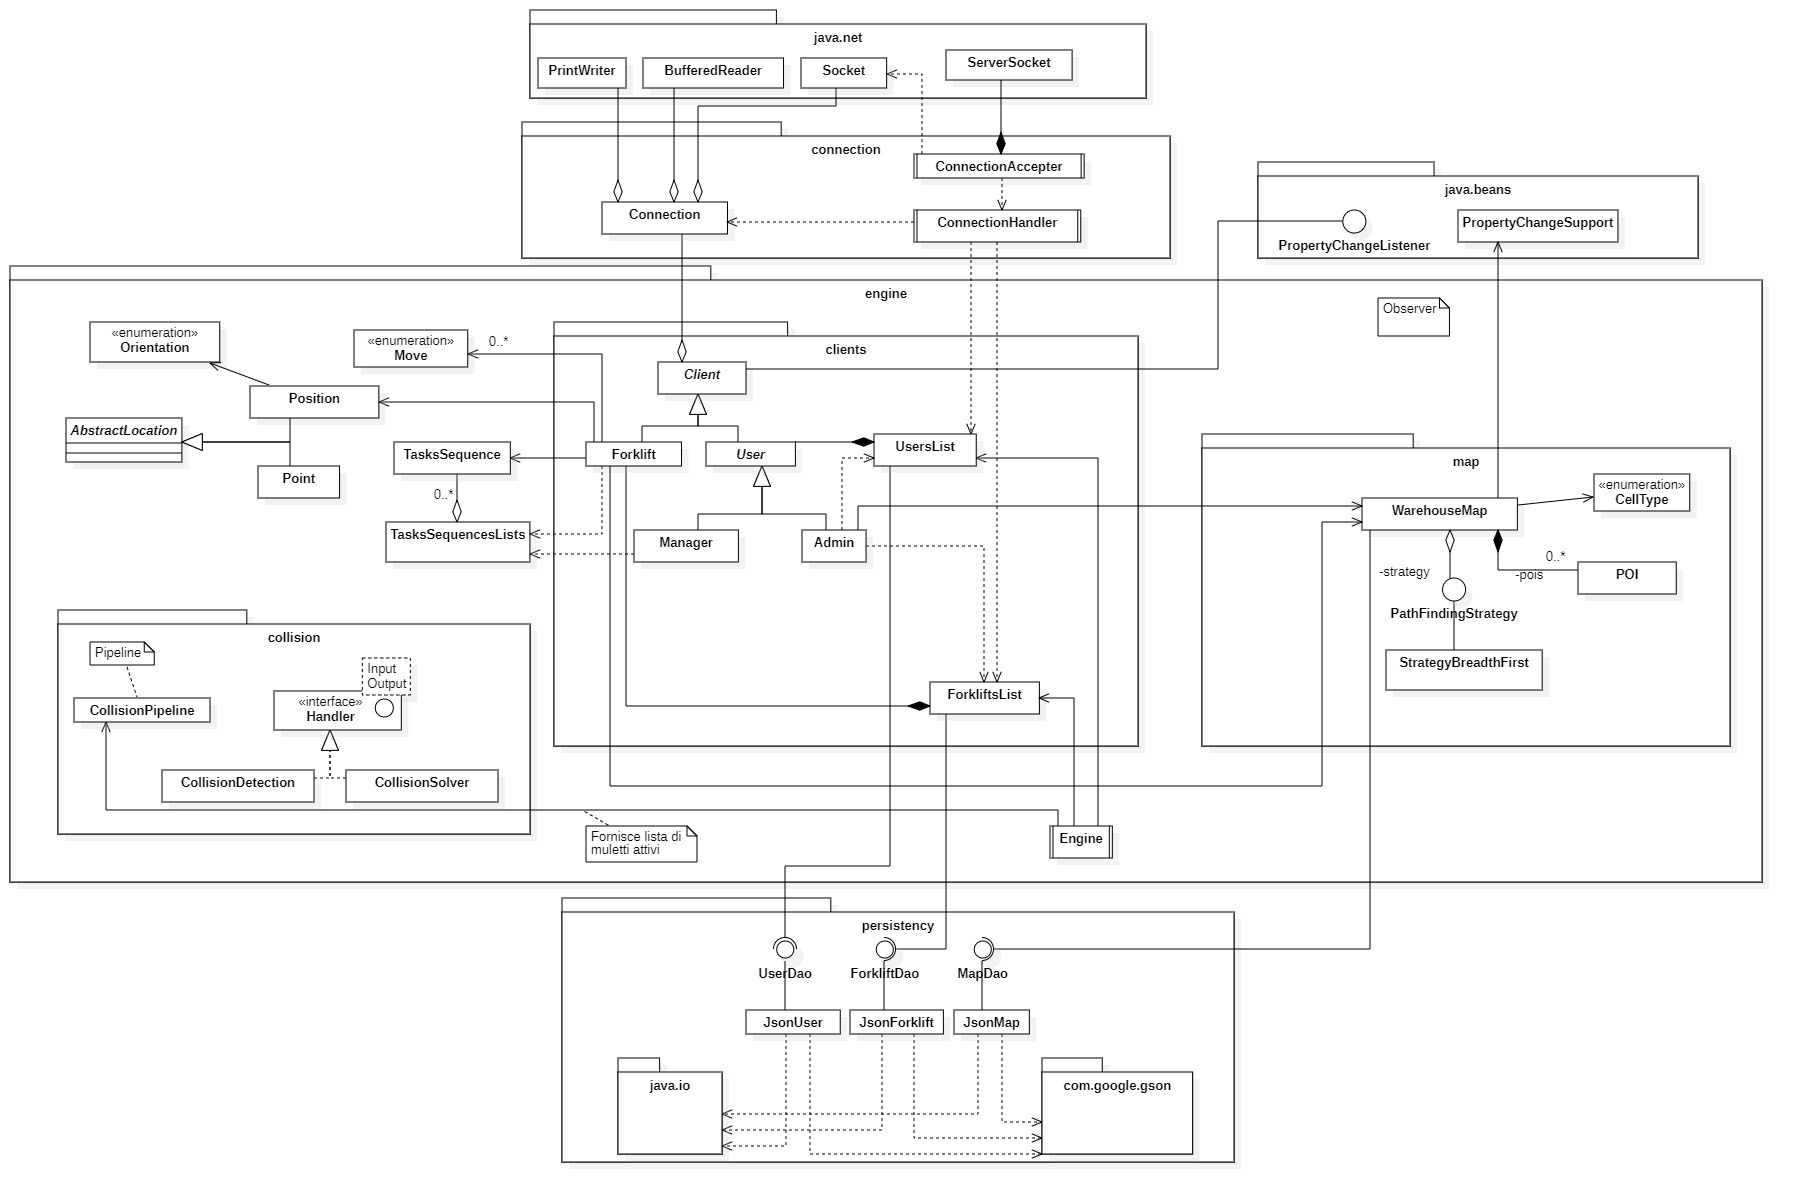
\includegraphics[scale=0.22]{res/diagrams/server/server_complessivo_minimal.jpg}
	\caption{Visione complessiva dell'architettura del server}
\end{figure}

Le sezioni che seguono illustrano la struttura di ogni layer.

\subsubsection{Communication layer}
\label{communication-layer}

\begin{figure}[H]
	\centering
	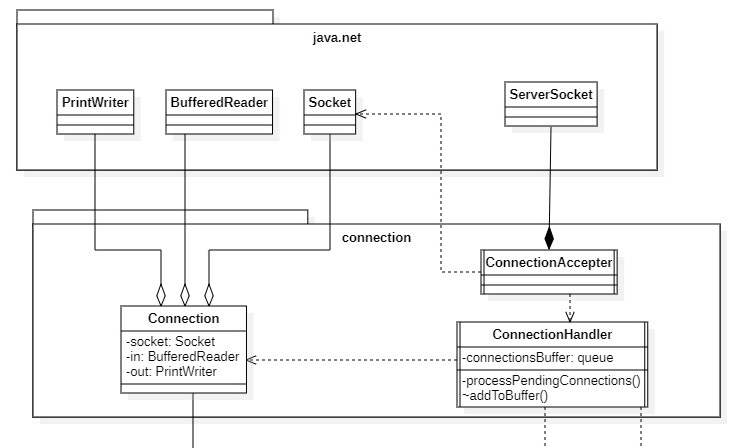
\includegraphics[scale=0.55]{res/diagrams/server/server_communication.jpg}
	\caption{Visione di dettaglio del Communication Layer}
\end{figure}


Questo layer si interfaccia con i client esterni e ha lo scopo di gestire la comunicazione con questi. In particolare, la classe \texttt{ConnectionAccepter} si occupa di accettare le nuove connessioni entranti tramite \texttt{ServerSocket}: essa esegue su un thread dedicato in modo da non bloccare le altre operazioni all'arrivo di una nuova connessione.

Per ogni nuova connessione, crea un oggetto \texttt{Socket} che passa a \texttt{ConnectionHandler}. Quest'ultima è una componente che esegue su un altro thread dedicato: rimane in attesa fino al risveglio determinato da \texttt{ConnectionAccepter}: una volta attivato, procede a svuotare il buffer di \texttt{Socket} per creare oggetti di tipo \texttt{Connection}, istanziando per ognuno i buffer di input e output. Segue quindi il processo di autenticazione dei muletti o degli utenti, al termine del quale \texttt{ConnectionHandler} torna in attesa.







\subsubsection{Business layer}

Nel Business layer risiede il nucleo di elaborazione dei dati ricevuti dal layer superiore: i domini principali di cui si occupa sono:
\begin{itemize}
	\item gestione della mappa e path finding;
	\item autenticazione dei client;
    \item elaborazione delle richieste;
	\item gestione delle tasks e dei POI;
	\item rilevazione e risoluzione delle collisioni.
\end{itemize}
Per facilitare la consultazione, lo studio di questo layer si concentra separatamente sui package di cui si compone. Per una visione dall'alto, riferirsi al diagramma complessivo all'inizio della sezione 5.1.



\clearpage
\paragraph{Clients}
\subparagraph*{ }

\begin{figure}[H]
	\centering
	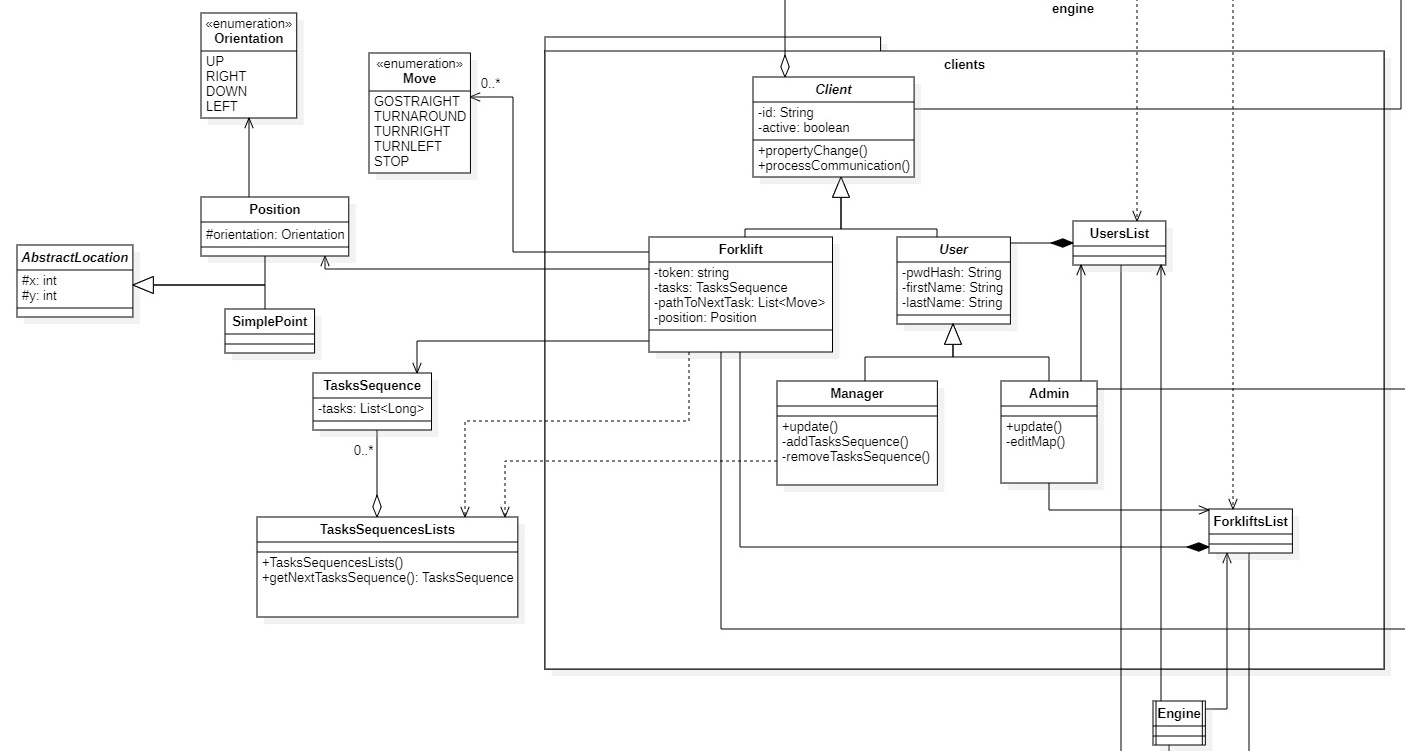
\includegraphics[scale=0.40]{res/diagrams/server/server_pack_clients.jpg}
	\caption{Visione di dettaglio del package Clients}
\end{figure}

La gerarchia dei \texttt{Client} prevede una prima suddivisione suddivisione tra \texttt{Forklift} e \texttt{User} (muletto e utente), gli \texttt{User} si specializzano ulteriormente in \texttt{Manager} (responsabile) e \texttt{Admin} (amministratore). Viene mantenuto a runtime lo stato di tutti i muletti e degli utenti registrati rispettivamente in \texttt{ForkliftsList} e \texttt{UsersList} così da ridurre le operazioni sulla persistenza.

I \texttt{Forklift} si caratterizzano dagli attributi:
\begin{itemize}
	\item \texttt{position}: rappresenta la posizione e orientamento attuali del muletto nella mappa;
	\item \texttt{tasks}: sequenza di task da compiere;
	\item \texttt{pathToNextTask}: una lista di mosse atte a raggiungere il prossimo POI (e quindi evadere la prossima task).
\end{itemize}

Notare che ogni \texttt{Client} possiede un attributo di tipo \texttt{Connection}, attraverso il quale viene regolata la comunicazione tramite Socket (per i dettagli si rimanda alle \S\ \ref{communication-layer} e \ref{communication-section}). Questo viene assegnato all'autenticazione e può cambiare un numero indefinito di volte, ogni qual volta che la connessione con il client verrà chiusa per qualsiasi ragione alla riconnessione questa verrà correttamente abbinata alla sua istanza.\\

La classe \texttt{Engine} è il cuore del motore di calcolo: essa esegue su un thread dedicato e tramite un timer scandisce l'esecuzione temporizzata dell'elaborazione. In particolare, interroga periodicamente \texttt{ForkliftsList} e \texttt{UsersList} con i seguenti obiettivi:
\begin{itemize}
	\item ricevere le nuove posizioni dai muletti;
	\item inviare le nuove informazioni agli utenti per la visualizzazione nel monitor real-time;
	\item rispondere ad eventuali altre richieste dell'iterazione precedente, avendo nel frattempo completato la loro elaborazione (calcolo percorso, aggiunta task, modifica mappa).
\end{itemize}
Dopodichè la \texttt{ForkliftsList} viene utilizzata dal modulo di rilevazione e gestione delle collisioni.

In questo layer si concentra l'utilizzo del framework Spring, utilizzato per gestire le dipendenze: alcune classi di utilizzo frequente e condiviso come \texttt{UsersList}, \texttt{ForkliftsList} e \texttt{TasksSequencesLists} (quest'ultima contenente tutte le liste di task inserite dal responsabile) vengono istanziate tramite \textit{Dependency Injection} sfruttando il meccanismo dei \textit{Bean} di Spring.




\paragraph{Mappa}
\subparagraph*{ }

\begin{figure}[H]
	\centering
	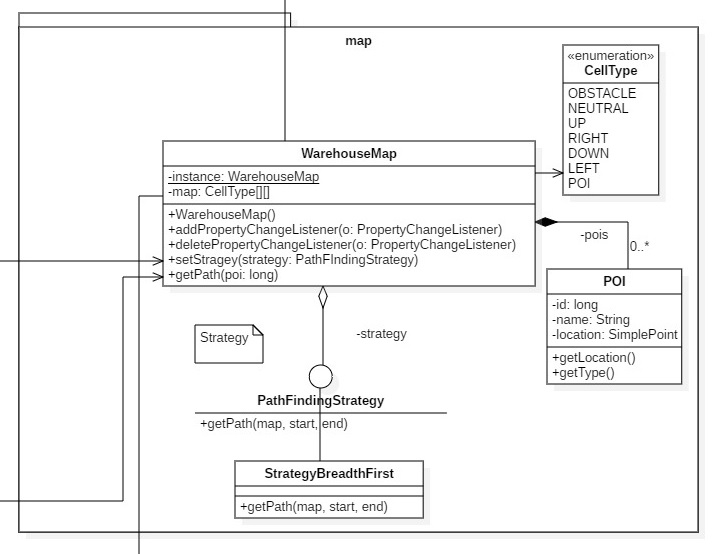
\includegraphics[scale=0.60]{res/diagrams/server/server_pack_map.jpg}
	\caption{Visione di dettaglio del package Map}
\end{figure}


La classe \texttt{WarehouseMap} contiene la rappresentazione della planimetria del magazzino: essa è rappresentata tramite una matrice di \texttt{CellType}, campo di tipo enumerazione che esprime le caratteristiche di ogni frazione spaziale. Alla mappa è associata una lista di POI, e per ognuno la relativa locazione.
Si osserva l'applicazione di alcuni design pattern:
\begin{itemize}
	\item \textbf{observer}: tramite \texttt{PropertyChangeSupport} e \texttt{PropertyChangeListener} di \texttt{java.beans} viene applicato il pattern \textit{observer}, definendo la \texttt{WarehouseMap} come Subject, e i \texttt{Client} come \textit{Observer}: essi verranno notificati ad ogni cambiamento della stessa in modo che possano comunicarlo tramite le connessioni, così da riflettere le modifiche ed aggiornare le interfacce grafiche che visualizzano la mappa;
	\item \textbf{strategy}: per l’algoritmo di path finding attualmente viene implementata una strategia di tipo \textit{breadth-first}, ma l’impostazione del pattern permette di aggiungere e variare dinamicamente eventuali altre implementazioni aggiunte in futuro. \texttt{WarehouseMap} assume il ruolo di \textit{context}, e i beneficiari sono i \texttt{Forklift}, i quali richiederanno il percorso ogni qualvolta si renderà necessario.
\end{itemize}





\paragraph{Collisioni}
\subparagraph*{ }

\begin{figure}[H]
	\centering
	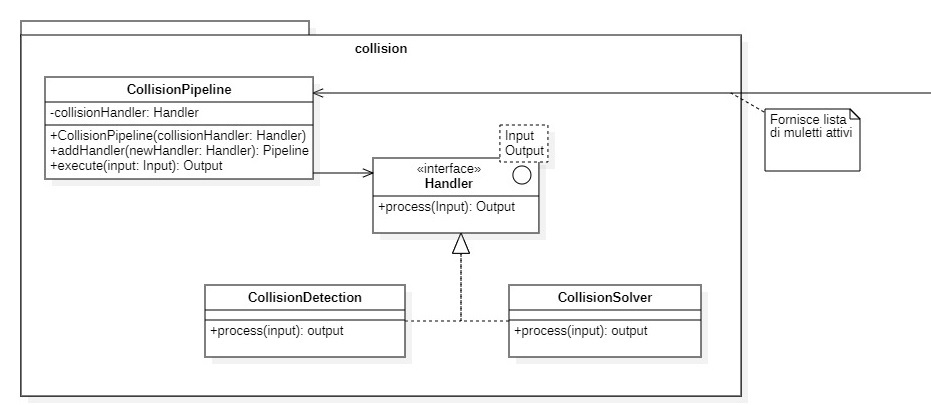
\includegraphics[scale=0.50]{res/diagrams/server/server_pack_collision.jpg}
	\caption{Visione di dettaglio del package Collision}
\end{figure}


Qui è contenuta la logica che gestisce le collisioni fra i muletti che circolano in guida autonoma all'interno del magazzino. L'elaborazione è scandita dal timer dell'\texttt{Engine}: ad ogni intervallo di tempo, vengono eseguite due operazioni sequenziali:
\begin{itemize}
	\item \textbf{rilevazione:} sulla base delle future mosse di ogni unità, vengono determinate le possibili collisioni;
	\item \textbf{risoluzione:} in caso vengano rilevate, vengono elaborate le mosse, da trasmettere alle unità coinvolte, che impediscano tali collisioni.
\end{itemize}
Le classi \texttt{CollisionDetector} e \texttt{CollisionSolver} incapsulano rispettivamente le due funzionalità elencate.

Viene applicato in questo contesto il design pattern \texttt{Pipeline}\footnote{Variante del pattern \textit{Chain Of Responsibility}: \url{https://java-design-patterns.com/patterns/pipeline/}}, che permette di definire vari \texttt{Handler} da comporre come catena di operazioni. La pipeline può essere poi eseguita (se necessario, come in questo caso, ripetutamente) con un comando che attiva i vari step sequenzialmente. Ogni \texttt{Handler} specifica i tipi del proprio parametro di input e di output: l'output di un \texttt{Handler} sarà l'input dell'\texttt{Handler} successivo.
In questo caso l'input sarà una struttura rappresentante muletti attivi con le loro posizioni e prossime mosse, mentre l'output un'altra struttura che ad ogni punto con collisione associ i muletti coinvolti e le azioni da intraprendere così da poterle comunicare.



\subsubsection{Persistence layer}

\begin{figure}[H]
	\centering
	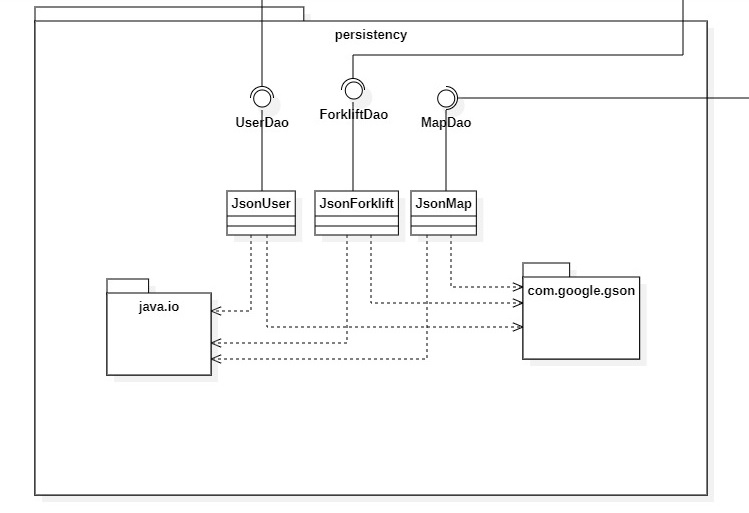
\includegraphics[scale=0.50]{res/diagrams/server/server_persistency.jpg}
	\caption{Visione di dettaglio del Persistence Layer}
\end{figure}

L'accesso a questo layer è regolato da 3 interfacce che gestiscono la persistenza delle tre tipologie di dati che vengono salvati:
\begin{itemize}
	\item i dati e le credenziali degli utenti;
	\item gli identificativi ed i token di autenticazione dei muletti;
	\item la rappresentazione della mappa.
\end{itemize}

Ogni interfaccia si rivolge alla relativa componente del layer superiore che conserva a runtime i dati impiegati nell'esecuzione. La presenza delle interfacce favorisce il disaccoppiamento tra i moduli e permette di estendere a tipi di persistenza alternativi. Attualmente è implementato il salvataggio dei dati su file di tipo .json, viene fatto uso della libreria standard java.io e GSON per gestire l'interazione con questo tipo di tecnologia.


\pagebreak
 %@Simone

	\subsection{Client}
\subsubsection{Diagrammi }

\begin{figure}[H]
	\centering
	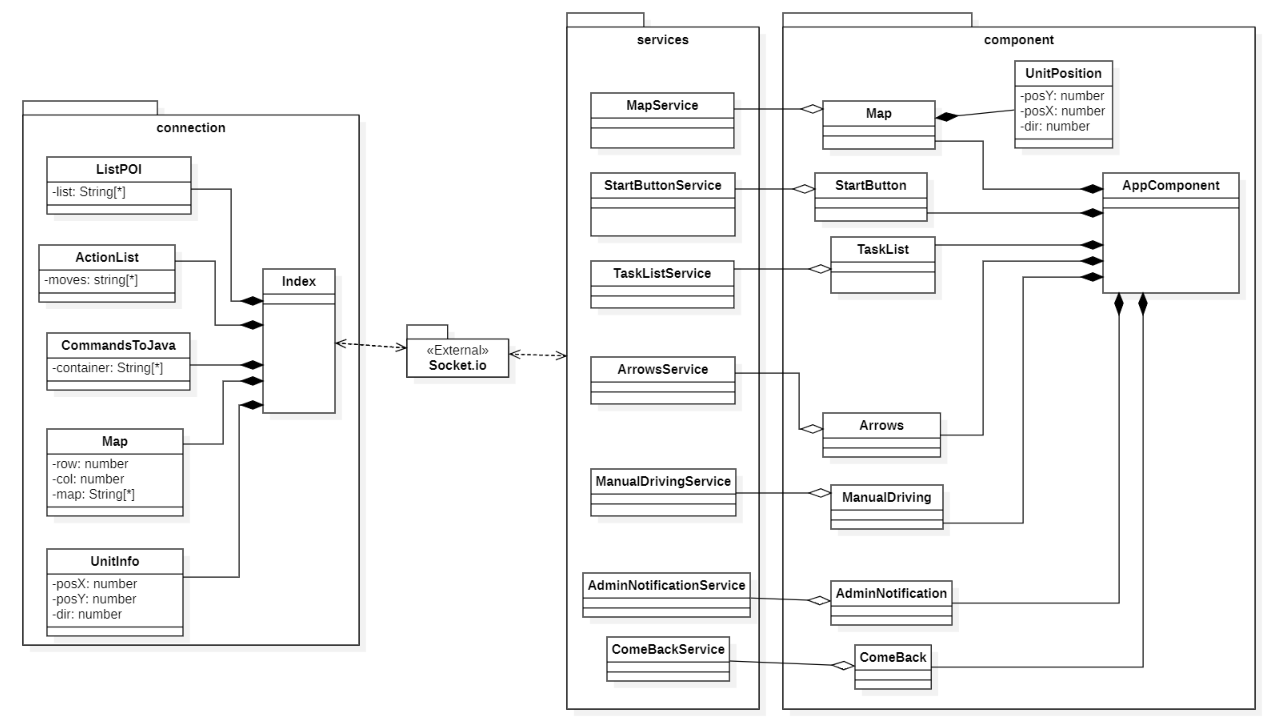
\includegraphics[scale=0.20]{res/images/UML_operatore.png}
	\caption{Diagramma UML delle classi per l'unità}
\end{figure}



 %@TeamFE

	\subsection{Comunicazione}



 %@Gregg - Intro - fatto

	\subsubsection{Diagrammi di sequenza} %@Alberto

	\clearpage
\subsubsection{Protocollo di comunicazione}
\label{comm-protocol}

Ogni stringa può contenere uno o più comandi, separati da ‘;' e ogni comando può avere 0 o più parametri, separati da ',’. \\
\textbf{Esempio sequenza:} \texttt{POS,1,1,0;PATH,1}

\pparagraph{Connessione: identificazione e login}
    Quando un client si connette deve essere identificato come tipo ed autenticato, perciò deve inviare separatamente ed in sequenza:
    \begin{enumerate}
        \item \textbf{TYPE: }\texttt{FORKLIFT} o \texttt{USER};
        \item \textbf{ID: } identificativo personale;
        \item \textbf{PWD/TOKEN: } password o token a seconda che sia rispettivamente un utente o un muletto.
    \end{enumerate}
    Quindi riceverà come risposta:
    \begin{itemize}

        \item nel caso di FORKLIFT: OK oppure FAIL,MSG

        \item nel caso di USER: OK,TYPE oppure FAIL,MSG

        \subitem -- dove TYPE indica il ruolo dell’utente (ADMIN o MANAGER)
    \end{itemize}
    dove MSG conterrà maggiori dettagli sulla causa.

    \subparagraph{Esempio connessione ed autenticazione muletto}
        Dato un muletto con id=f1 e token=abcdef:
        \begin{itemize}
            \item invia: \texttt{FORKLIFT\textbackslash nf1\textbackslash nabcdef};

            \item riceve: \texttt{OK} oppure \texttt{FAIL,messaggioErrore}
        \end{itemize}


        Funzionamento analogo per gli utenti con password al posto di token.

\pparagraph{Enumerazioni}
    In seguito si farà riferimento più volte ai diversi tipi enum presenti nella logica di business, per cui segue un riassunto:


    \begin{table}[h!]
        \centering
        \begin{tabular}{|c|c|c|c|c|}
            \hline
            \rowcolorhead
            \multicolumn{5}{|c|}{\headertitle{ENUM}}\\
            \hline
            \rowcolorhead
            \headertitle{↓Val \textbackslash{} Enum→} & \headertitle{PoiType} & \headertitle{Move}       & \headertitle{Orientation} & \headertitle{CellType} \\
            0          & LOAD    & GOSTRAIGHT & UP          & OBSTACLE \\
            1          & UNLOAD  & TURNAROUND & RIGHT       & NEUTRAL \\
            2          & EXIT    & TURNRIGHT  & DOWN        & UP \\
            3          & --      & TURNLEFT   & LEFT        & RIGHT \\
            4          & --      & STOP       & --          & DOWN \\
            5          & --      & --         & --          & LEFT \\
            6          & --      & --         & --          & POI \\ [1ex]
            \hline
        \end{tabular}
        \caption{Riepilogo enumerazioni}
    \end{table}
\newcommand{\tabitem}{~~\llap{\textbullet}~~}

\clearpage
\pparagraph{Comandi clients → server}
Per i comandi di risposta, controllare i corrispondenti in \S\ \ref{commands-server-client}
    \begin{table}[h!]
        \centering
        \begin{tabular}{|c|p{8cm}|c|}
            \hline
            \rowcolorhead
            \multicolumn{3}{|c|}{\headertitle{FORKLIFTS → SERVER}}\\
            \hline
            \rowcolorhead
            \headertitle{Comando} & \headertitle{Descrizione} & \headertitle{Risposta} \\
            \hline
            \texttt{POS,X,Y,DIR} & Posizione attuale del muletto, considerando la mappa come una matrice:
            \begin{itemize}
                \item X: riga della matrice
                \item Y: colonna ““
                \item DIR: orientamento assoluto secondo enum Orientation
            \end{itemize}

            & -- \\
            \texttt{LIST} & Richiede nuova lista di task da completare & \texttt{LIST,...} \\

            \texttt{PATH,C} & Richiede il percorso migliore per raggiungere il POI della task corrente a partire dalla posizione attuale. Se C=1 rimuove la task e passa alla successiva & \texttt{PATH,...} \\

            \hline
        \end{tabular}
        \caption{Comandi clients → server | Forklifts}
    \end{table}

    \begin{table}[h!]
        \centering
        \begin{tabular}{|c|p{8cm}|c|}
            \hline
            \rowcolorhead
            \multicolumn{3}{|c|}{\headertitle{USER generico → SERVER}}\\
            \hline
            \rowcolorhead
            \headertitle{Comando} & \headertitle{Descrizione} & \headertitle{Risposta} \\
            \hline
            \texttt{EDIT,T,PAR} & Modifica dati del proprio profilo
            \begin{itemize}
                \item T: NAME/LAST/PWD

                \item PAR: nuova valore per T
            \end{itemize}
             & -- \\

             \texttt{LOGOUT} & Richiesta di disconnessione & -- \\

            \hline


        \end{tabular}
        \caption{Comandi clients → server | User generico}
    \end{table}

    \begin{table}[h!]
        \centering
        \begin{tabular}{|c|p{8cm}|c|}
            \hline
            \rowcolorhead
            \multicolumn{3}{|c|}{\headertitle{MANAGER → SERVER}}\\
            \hline
            \rowcolorhead
            \headertitle{Comando} & \headertitle{Descrizione} & \headertitle{Risposta} \\
            \hline
            \texttt{ADL,P1,P2,…} & Aggiunge una nuova lista di task
            \begin{itemize}

                \item P1..: id dei poi che compongono la lista
            \end{itemize}
            & \texttt{ADL,...} \\

            \texttt{RML,ID} & Richiede la cancellazione della lista con id=ID & \texttt{RML,...} \\

            \hline
        \end{tabular}
        \caption{Comandi clients → server | User Manager (Responsabile)}
    \end{table}

    %\begin{table}[h!]
        %\centering
        \begin{longtable}[h!]{|c|p{8cm}|c|}
            %\endfirsthead
            \hline
            \rowcolorhead
            \multicolumn{3}{|c|}{\headertitle{ADMIN → SERVER}}\\
            \hline
            \rowcolorhead
            \headertitle{Comando} & \headertitle{Descrizione} & \headertitle{Risposta} \\
            \hline
            \endhead

            \texttt{MAP,R,C,SEQ} & Nuova planimetria
            \begin{itemize}
                \item R: num righe
                \item C: “ colonne
                \item SEQ: sequenza di interi corrispondenti all’enum CellType rappresentanti stati di una cella, indicanti la nuova planimetria, elencati per righe
            \end{itemize}
            & \texttt{MAP,...} \\

            \texttt{CELL,X,Y,A[,T,NAME]} & Modifica una cella, la parte tra [ ] è presente solo in caso di POI
            \begin{itemize}
                \item X e Y riga e colonna della matrice

                \item A: numero rappresentante l'azione  da intraprendere, corentemente con CellType
            \end{itemize}

            Solo nel caso di POI:
            \begin{itemize}
                \item T: tipo di POI secondo PoiType

                \item NAME: stringa di caratteri da associare al POI
            \end{itemize}
            & \texttt{CELL,...} \\

            \texttt{ADU,T,NAME,LAST} & aggiunge nuovo utente
            \begin{itemize}
                \item T: tipo (ADMIN o MANAGER)

                \item NAME e LAST: rispettivamente nome e cognome
            \end{itemize}
            & \texttt{ADU,...} \\

            \texttt{RMU,ID} & Rimuove l’utente con id=ID & \texttt{RMU,...} \\

            \texttt{EDU,ID,A,PAR} & Modifica l’utente con id=ID, con
            \begin{itemize}
                \item A: azione da intraprendere tra:

                    \subitem -- NAME: modifica nome

                    \subitem -- LAST: modifica cognome

                    \subitem -- RESET: esegue reset della password
                \item PAR: nuovo valore da assegnare (assente in caso di reset)
            \end{itemize}
            & \texttt{EDU,...} \\

            \texttt{ADF,ID} & Aggiunge nuovo muletto. ID: stringa che si vuole assegnare come identificativo al nuovo muletto (NON sarà più modificabile) & \texttt{ADF,...} \\

            \texttt{RMF,ID} & Rimuove il muletto con id=ID & \texttt{RMF,...} \\

            \texttt{LISTF} & Richiede lista di tutti i muletti registrati & \texttt{LISTF,...} \\

            \texttt{LISTU} & Richiede lista di tutti gli utenti registrati & \texttt{LISTU,...} \\
            \hline
        \hiderowcolors
        \caption{Comandi clients → server | User Admin (Amministratore)}\\
        \showrowcolors
        \end{longtable}

    %\end{table}

\clearpage
\pparagraph{Comandi server → clients}
\label{commands-server-client}
    Tutti i comandi che possono ritornare un esito positivo o negativo hanno 2 varianti:
    \begin{itemize}
        \item \texttt{CMD,OK,MORE}: successo, eventualmente MORE contiene parametri di risposta aggiuntivi
        \item \texttt{CMD,FAIL,MSG}: fallimento, MSG contiene maggiori informazioni sulle cause.
    \end{itemize}

    \begin{table}[h!]
        \centering
        \begin{tabular}{|c|p{8cm}|c|}
            \hline
            \rowcolorhead
            \multicolumn{3}{|c|}{\headertitle{SERVER → CLIENTS generici}}\\
            \hline
            \rowcolorhead
            \headertitle{Comando} & \headertitle{Descrizione} & \headertitle{Risposta} \\
            \hline
            \texttt{MAP,R,C,SEQ} & Indica la planimetria
            \begin{itemize}
                \item R e C: numero di righe e colonne

                \item SEQ: sequenza di interi corrispondenti all’enum CellType rappresentanti stati di una cella, indicanti la nuova planimetria, elencati per righe
            \end{itemize}
            & --\\
            \texttt{POI,N,X,Y,T,ID,NAME} & Rappresenta tutti i poi, la parte da X in poi si ripete per ogni POI
            \begin{itemize}
                \item N: num totale POI

                \item X,Y e T posizione nella matrice e tipo secondo PoiType

                \item ID e NAME: rispettivamente identificativo e nome del POI
            \end{itemize}
            & -- \\

            \hline
        \end{tabular}
        \caption{Comandi server → clients | generici per tutti i client}
    \end{table}

    \begin{table}[h!]
        \centering
        \begin{tabular}{|c|p{8cm}|c|}
            \hline
            \rowcolorhead
            \multicolumn{3}{|c|}{\headertitle{SERVER → FORKLIFT}}\\
            \hline
            \rowcolorhead
            \headertitle{Comando} & \headertitle{Descrizione} & \headertitle{Risposta} \\
            \hline
            \texttt{ALIVE} & Ha lo scopo primario di verificare l’integrità della connessione ed ha come effetto l’ottenimento della nuova posizione. Se l’invio fallisce il muletto corrispondente viene considerato disconnesso, l’oggetto Connection relativo verrà chiuso e distrutto e il muletto dovrà riautenticarsi. Si presuppone che questo non si muova più finché la connessione non viene ristabilita, in quanto i suoi spostamenti sarebbero sconosciuti al server e questo non potrebbe intervenire per evitare eventuali collisioni.

            Ad esso possono seguire ulteriori comandi o risposte a comandi precedente, secondo la sintassi generale per cui separati da ';'
            & \texttt{POS,...} \\

            \texttt{LIST,ID1,ID2…} & Invia lista di task assegnate. ID1.. sono gli id dei POI da raggiungere & -- \\

            \texttt{PATH,SEQ} & Invia il percorso per raggiungere il prossimo POI, composto da mosse successive secondo Move & -- \\

            \texttt{STOP,N} & Richiede lo stop immediato del muletto per N istanti, che verranno contati alle ricezioni dei futuri ALIVE. Se N=0 stop indefinito fino alla ricezione di \texttt{START}. & -- \\
            \texttt{START} & consente ad un muletto fermato a tempo indeterminato di ripartire & -- \\

            \hline
        \end{tabular}
        \caption{Comandi server → clients | Forklifts (muletti)}
    \end{table}

    \begin{table}[h!]
        \centering
        \begin{tabular}{|c|p{8cm}|c|}
            \hline
            \rowcolorhead
            \multicolumn{3}{|c|}{\headertitle{SERVER → USER generico}}\\
            \hline
            \rowcolorhead
            \headertitle{Comando} & \headertitle{Descrizione} & \headertitle{Risposta} \\
            \hline
            \texttt{UNI,N,ID1,X1,Y1,D1} & Indica le posizioni di tutti i muletti. Da ID1 in poi si ripete per ogni muletto
            \begin{itemize}
                \item N: num totale dei muletti attivi per i quali si sta ricevendo la posizione

                \item IDn: id del muletto n

                \item Xn, Yn e Dn: posizione rispetto alla matrice e orientamento secondo Orientation del muletto IDn.
            \end{itemize}
            Se l'invio di questo fallisce, l'utente viene considerato disconnesso.
            & -- \\

            \texttt{LIST,IDF,N,IDP1,IDP2…} & Indica la lista di task presa in carico da un muletto
            \begin{itemize}
                \item IDF: id del muletto a cui ci si sta riferendo

                \item N: numero di task prese in carico

                \item IDP1…: sequenza di id dei POI da raggiungere
            \end{itemize}
            & -- \\


            \hline
        \end{tabular}
        \caption{Comandi server → clients | User generico}
    \end{table}


    \begin{table}[h!]
        \centering
        \begin{tabular}{|c|p{8cm}|c|}
            \hline
            \rowcolorhead
            \multicolumn{3}{|c|}{\headertitle{SERVER → MANAGER}}\\
            \hline
            \rowcolorhead
            \headertitle{Comando} & \headertitle{Descrizione} & \headertitle{Risposta} \\
            \hline
            \texttt{ADL,OK,ID} & Conferma aggiunta nuova lista di task. ID indica l'identificativo della nuova lista & -- \\

            \texttt{ADL,FAIL,MSG} & Segnala errore nella creazione di una nuova lista di task. & -- \\
            \multicolumn{3}{|c|}{Funzionamento analogo per \texttt{RML}}\\


            \hline
        \end{tabular}
        \caption{Comandi server → clients | Utente Manager (responsabile)}
    \end{table}

    \begin{table}[h!]
        \centering
        \begin{tabular}{|c|p{8cm}|c|}
            \hline
            \rowcolorhead
            \multicolumn{3}{|c|}{\headertitle{SERVER → ADMIN}}\\
            \hline
            \rowcolorhead
            \headertitle{Comando} & \headertitle{Descrizione} & \headertitle{Risposta} \\
            \hline
            \texttt{MAP,OK} & Conferma successo modifica mappa & -- \\
            \texttt{MAP,FAIL,MSG} & Modifica mappa fallita & -- \\
            \multicolumn{3}{|c|}{Analogamente a quelli sopra, stesso discorso vale per: \texttt{CELL, RMU, RMF}} \\
            \texttt{ADU,ID,PWD} & In risposta alla creazione di un utente

            \begin{itemize}
                \item ID che rappresenta il nuovo utente

                \item PWD password temporanea per il nuovo utente, il quale è tenuto a cambiarla tempestivamente
            \end{itemize}
            & -- \\

            \texttt{EDU,OK[,PWD]} & Modifica utente avvenuta con successo. PWD contiene la nuova password in caso di richiesta di reset. Anche in questo caso, l'utente una volta ricevuta la password dall'admin è tenuto a reimpostarla.
            & --\\

            \texttt{EDU,FAIL,MSG} & Modifica utente fallita
            & -- \\

            \texttt{ADF,OK,TOKEN} & Aggiunta di un nuovo muletto avvenuta con successo. Il TOKEN serve per la configurazione del nuovo muletto sul dispositivo client che verrà associato alla nuova unità & --\\
            \texttt{ADF,FAIL,MSG} & Aggiunta nuovo muletto fallita (esiste già muletto con l'id richiesto) & -- \\

            \texttt{LISTF,N,ID1,T1,ID2,T2…} & In risposta alla richiesta della lista dei muletti:
            \begin{itemize}
                \item N: num totale muletti

                \item IDn, Tn: rispettivamente id e token del muletto n
            \end{itemize}
            & -- \\

            \texttt{LISTU,N,UN1,UL1,R1…} & In risposta alla richiesta della lista degli utenti:
            \begin{itemize}
                \item N: num totale utenti

                \item UN…: rispettivamente nome, cognome e ruolo
            \end{itemize}
            & -- \\


            \hline
        \end{tabular}
        \caption{Comandi server → clients | Utente Admin (amministratore)}
    \end{table}


\begin{comment}
\begin{longtable}[h!]{|p{2cm}|p{8cm}|p{2cm}|}
\hline
\rowcolorhead
\multicolumn{3}{|c|}{\headertitle{FORKLIFTS}}\\
\hline
\rowcolorhead
\headertitle{Comando} & \headertitle{Descrizione} & \headertitle{Risposta} \\
\hline
POS,X,Y,DIR & posizione attuale del muletto, considerando la mappa come una matrice:\newline
\begin{itemize}
\item     X: riga della matrice
\item     Y: colonna ““
\item     DIR: orientamento assoluto secondo enum Orientation
\end{itemize}

& -- \\
LIST & richiede nuova lista di task da completare & LIST... \\




\caption{prova}
\end{longtable}
\end{comment}














 %@Gregg
	\pagebreak

    %\begin{comment}
        	\section{Estendere PORTACS}
In questa sezione verranno riportate tutte quelle informazioni utili ad una semplice e corretta estensione del prodotto PORTACS. Possono essere estensioni legate sia a nuovi algoritmi e framework, più efficaci o efficienti, che a nuove categorie di sotto-sistemi di PORTACS.














 %Tex - intro

        \subsection{Algoritmo alternativo per il path finding}
Si può aggiungere un algoritmo alternativo di path finding, oltre a quello già implementato con una strategia breadth first (in ampiezza).
Per farlo, bisogna creare una classe che implementi l'interfaccia \texttt{PathfindingStrategy}. Implementando questa interfaccia, viene creata una nuova strategia, e l'unica cosa necessaria da fare è implementare il metodo pubblico \texttt{getPath}, in quanto unico metodo utilizzato dall'esterno, che ritorna il percorso dal punto start a end sulla mappa, fatto di una list di moves (il nostro campo enum).
La strategia può essere cambiata tramite il metodo \texttt{setStrategy} nella classe \texttt{WareHouseMap} e dunque cambiare quella di default nella configurazione di Spring, oppure si può aggiungere un'operazione per l'amministratore per cambiare quella di default a run-time.
 %@Gregg

        \subsection{Introdurre nuove tipologie di utenti}


\subsubsection{Lato server} %@Gregg

        \subsubsection{Lato client}
Per introdurre nuovi tipi di utente basterà creare un nuovo package dentro \texttt{Connection} lato Node del sistema, inserendo tutte le funzionalità necessarie al tipo d'utente. \\Successivamente bisognerà implementare le corrispondenti parti nel package \texttt{Services} e \texttt{Component} di Angular per la visualizzazione. \\Infine bisognerà inserire il nuovo tipo di utente dentro la classe di \texttt{Login}. %@TeamFE

        \subsection{Implementare tipi di persistenza alternativi}
Le interfacce \textit{User}, \textit{Forklist} e Mapdataou danno informazioni sulla persistenza di utenti, muletti e mappa. Per implementare un nuovo tipo di persistenza bisogna creare una classe, implementando una di questa 3 interfacce, in base alla tipologia, e implementare i metodi richiesti dall'interfaccia.
Similmente all'algoritmo di \textit{pathfinding}, per settare questo tipo di persistenza bisogna passare per la configurazione Spring, per la gestione delle \textit{dependency injection}. %@Gregg

        \subsection{Modificare handler nell'algoritmo di gestione delle collisioni} %@Simone
        \pagebreak
    %\end{comment}



\end{document}
